%!TEX program = xelatex
% 完整编译: xelatex -> biber/bibtex -> xelatex -> xelatex
\documentclass[lang=cn,11pt,a4paper]{elegantpaper}

\title{有限元第一次编程作业}
\author{W Huang}
\date{\zhtoday}


% 本文档命令
\usepackage{array}
\usepackage{float}
\usepackage{multirow}
\newcommand{\ccr}[1]{\makecell{{\color{#1}\rule{1cm}{1cm}}}}

\begin{document}

\maketitle

\section{有限元推导}

求解PDE
\begin{equation}
    \left\{
        \begin{array}{l}
            -\Delta u + u = f,\quad \text{in}\;\Omega,\\
            \mathbf{n}\cdot \nabla u = 0,\quad \text{on}\;\partial\Omega.
        \end{array}
    \right.
\end{equation}

其中区域$\Omega=[0,1]^2$,取精确解:
\begin{equation}
    u(x,y)=\cos(\pi x)\cos(\pi y).
\end{equation}

导出右端项:
\begin{equation}
    f(x,y)=(2\pi^2+1)\cos(\pi x)\cos(\pi y).
\end{equation}

变分公式:求$u\in H^1(\Omega)$,使得,
\begin{equation}
    (u,v)+(\nabla u,\nabla v)=(f,v),\quad \forall v\in H^1(\Omega).
\end{equation}

使用三角网格$\mathcal{T}_h$,取$\mathcal{P}_1$元,有限元逼近空间为:
\begin{equation}
    V_h=\{u_h\in C(\bar{\Omega}):u_h|_\mathcal{K}\in\mathcal{P}_1,\;\forall \mathcal{K}\in\mathcal{T}_h\}\subset H^1(\Omega).
\end{equation}

求得的数值解$u_h\in V_h$可写为:
\begin{equation}
    u_h=\sum_{j=1}^N U_j \Phi_j.
\end{equation}

其中$N$为顶点个数,$\Phi_j$为顶点$j$的线性节点基函数。我们需要装配离散系统
\begin{equation}
    AU=F.
\end{equation}

其中,
\begin{align}
    A_{ij}&=(\Phi_i,\Phi_j)+(\nabla \Phi_i, \nabla \Phi_j),\quad i,j=1,...,N,\\
    F_i&=(\Phi_i,f),\quad i=1,...,N.
\end{align}

积分需要遍历所有函数值非零的三角形单元,将结果累加。在每个三角形中,积分值由二阶Gauss quadrature formula计算,由于我们采用的是$P_1$元,因此这样算出来的$(\Phi_i,\Phi_j)$与$(\nabla \Phi_i, \nabla \Phi_j)$都是精确的。

\section{数值测试}

用deal.ii自带的函数生成正方形网格,再进行三角化,生成米字形三角网格。按上节所述方式装配离散系统,用deal.ii的共轭梯度求解器解离散系统,当代数误差达到$10^{-6}||F||_2$时停止迭代,最终结果如下。(米字形网格的误差分布非常有意思)

\begin{figure}[H]
    \centering
    \begin{minipage}[t]{0.4\textwidth}
        \centering
        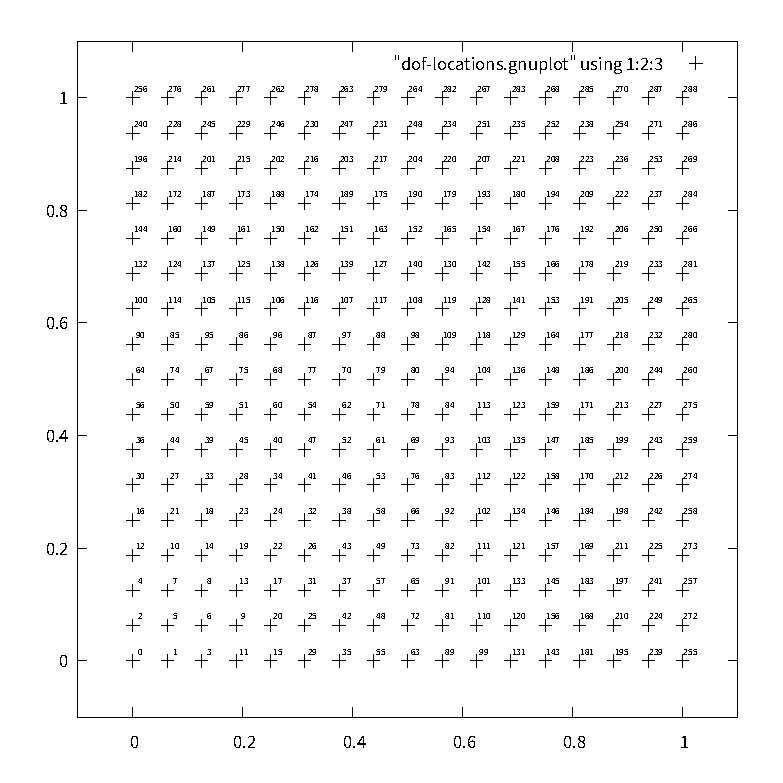
\includegraphics[width=0.9\linewidth]{fig/dof-locations.eps}
        \caption{$h=\frac{1}{16}$时的网格点编号}
    \end{minipage}
    \hspace{1em}
    \begin{minipage}[t]{0.4\textwidth}
        \centering
        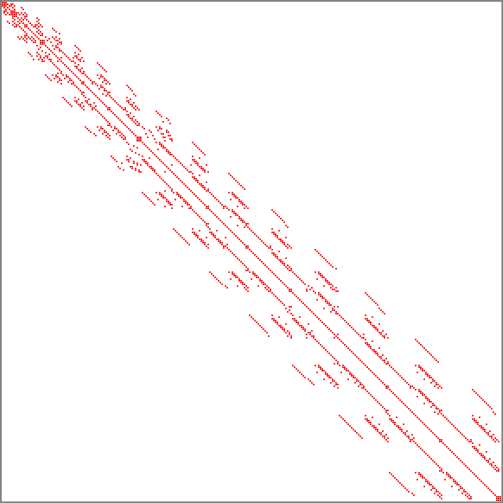
\includegraphics[width=0.8\linewidth]{fig/sparsity-pattern.png}
        \caption{$h=\frac{1}{16}$时得到的离散系统}
    \end{minipage}
\end{figure}

\begin{figure}[H]
    \centering
    \begin{minipage}[t]{0.48\textwidth}
        \centering
        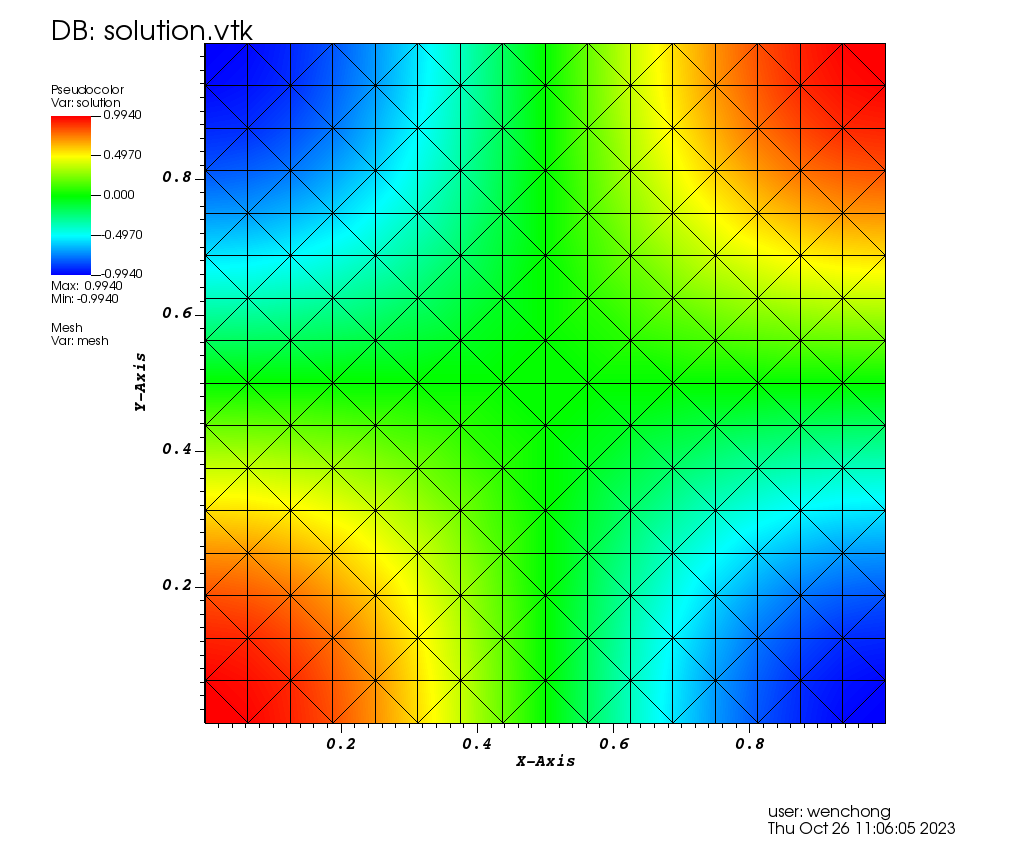
\includegraphics[width=\linewidth]{fig/solution.png}
        \caption{$h=\frac{1}{16}$时的数值解}
    \end{minipage}
    \begin{minipage}[t]{0.48\textwidth}
        \centering
        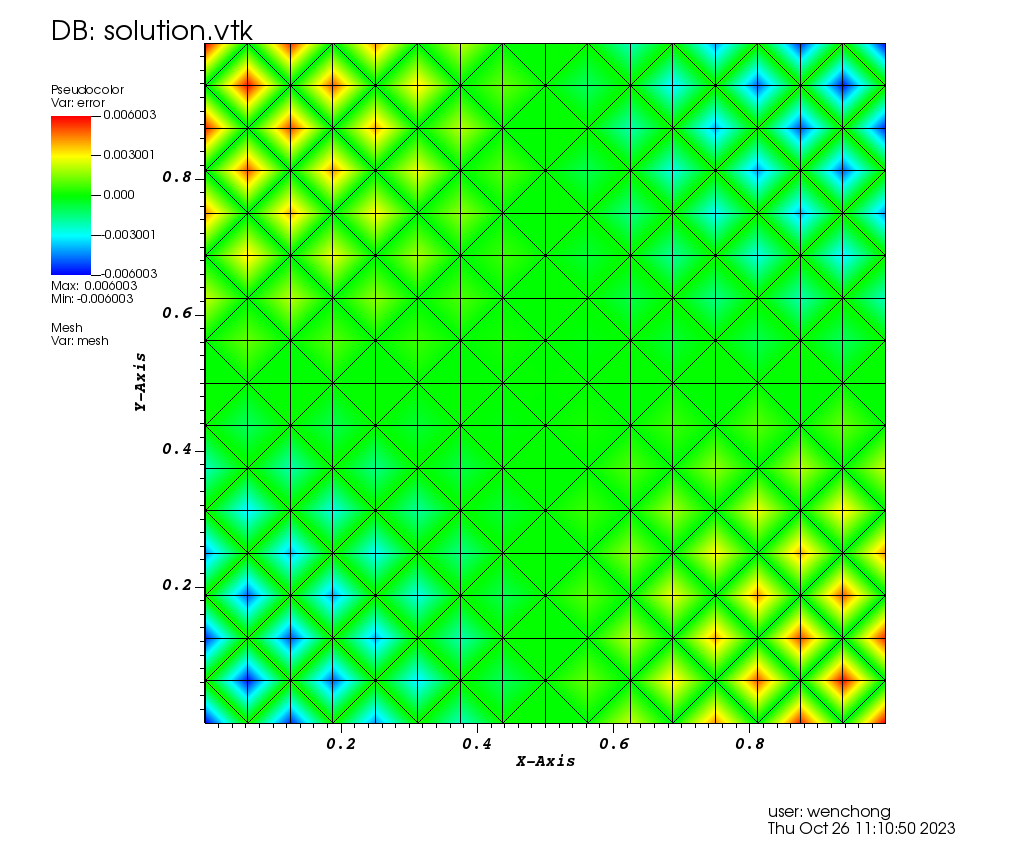
\includegraphics[width=\linewidth]{fig/error.png}
        \caption{$h=\frac{1}{16}$时数值解与真解的误差}
    \end{minipage}
\end{figure}

\begin{table}[H]
    \centering
    \begin{tabular}{|c|c|c|c|c|c|c|c|}
    \hline
    $h$                    & $\frac{1}{16}$ & Rate & $\frac{1}{32}$ & Rate & $\frac{1}{64}$ & Rate & $\frac{1}{128}$ \\ \hline
    $||u-u_h||_{L_1}$      & 0.00385344     & 2.00 & 0.000965871    & 2.00 & 0.00024153     & 2.00 & 6.03922e-05     \\ \hline
    $||u-u_h||_{L_2}$      & 0.00451671     & 2.00 & 0.0011314      & 2.00 & 0.00028299     & 2.00 & 7.07562e-05     \\ \hline
    $||u-u_h||_{L_\infty}$ & 0.0380602      & 1.99 & 0.00960736     & 2.00 & 0.00240764     & 2.00 & 0.000602272     \\ \hline
    $|u-u_h|_{H_1}$        & 0.205241       & 1.00 & 0.102761       & 1.00 & 0.0513983      & 1.00 & 0.0257014       \\ \hline
    $||u-u_h||_{H_1}$      & 0.205291       & 1.00 & 0.102768       & 1.00 & 0.0513991      & 1.00 & 0.0257015       \\ \hline
    CPU Time (s)           & 0.186          &      & 0.391          &      & 1.221          &      & 4.782           \\ \hline
    \end{tabular}
\end{table}

误差范数用积分计算,积分值在每个三角形单元里都由二阶Gauss quadrature formula计算。完全符合理论分析的结果。

\appendix
%\appendixpage
\addappheadtotoc

\end{document}
